\chapter{Introduction to Graphs}

Some data is easier to work with if we imagine it as a set of
\newterm{nodes} connected by \newterm{edges}.  For example, on some
social networks, each user can follow any number of other users.  We
can think of each user as a node, and the edge points from the user who
follows to the user they follow:\index{graph}\index{edge}\index{node}

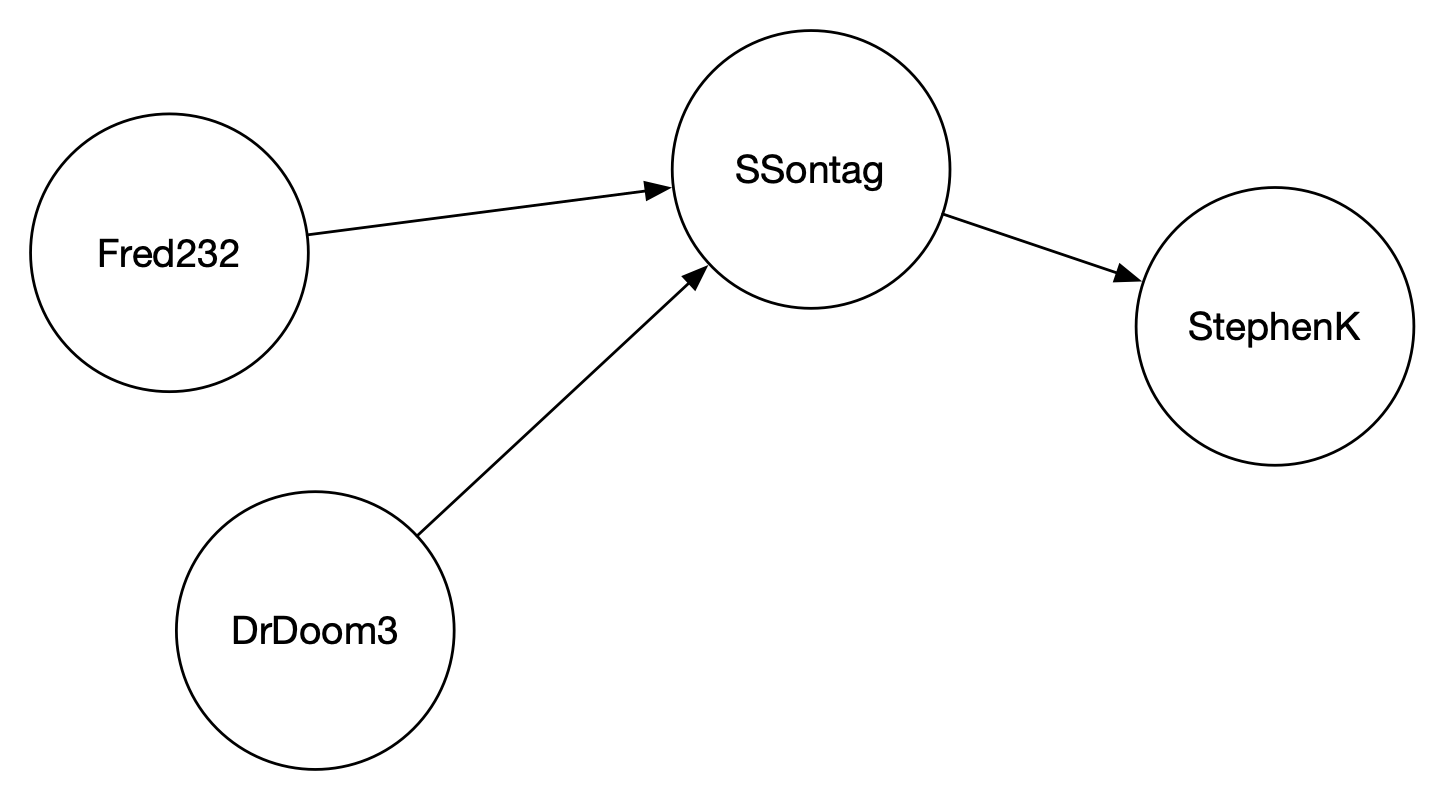
\includegraphics[width=0.7\textwidth]{simpledirected.png}

This diagram shows four users and three follows.  Following is a
directed relationship: Fred232 follows SSontag, but SSontag doesn't
follow Fred232.  So we would way that this is a \newterm{directed
  graph} with four nodes and three edges.\index{graph!directed}

There are also undirected graphs. For example, you can imagine a
graph that represents big data lines between cities.  All the big data
lines allow communications in both directions:\index{graph!undirected}

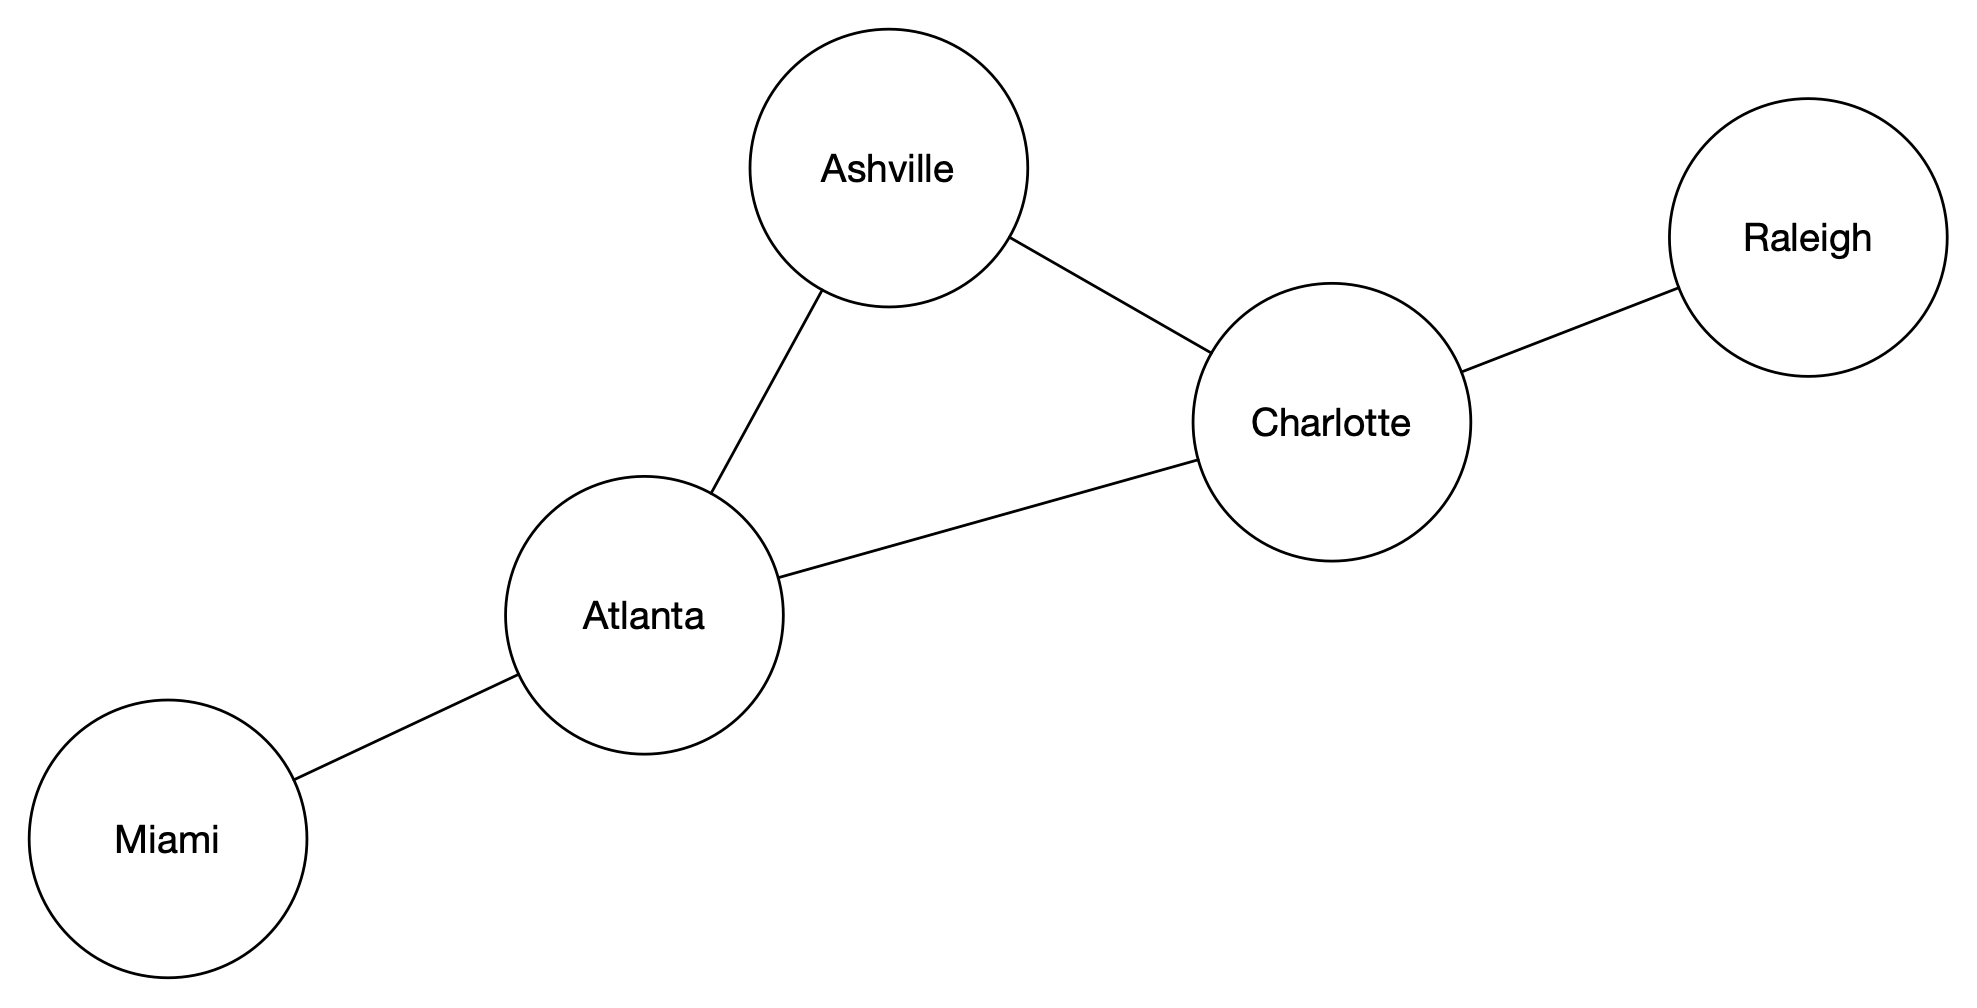
\includegraphics[width=0.7\textwidth]{simpleundirected.png}

The arrows are gone; if data can flow from Charlotte to Raleigh, then
data can flow from Raleigh to Charlotte.

There is a whole branch of mathematics called \newterm{Graph Theory}
that studies the properties of graphs.  Here are two questions that we
might ask about this graph:
\begin{itemize}
\item What is the shortest number of edges that we would need to follow to get from Miami to Raleigh?
\item Does the graph have any paths where you could end up where you
  started? This is called a \newterm{cycle}.  This graph has one
  cycle: Atlanta $\rightarrow$ Asheville $\rightarrow$ Charlotte
  $\rightarrow$ Atlanta.
\end{itemize}\index{graph theory}

There are even database systems that are specifically designed to hold
and analyze graph data. Not surprisingly, these are called
\newterm{Graph Databases}.\index{graph!database}

Some graphs are \newterm{connected}: You can get from one node to any
other node by following edges.  Is this graph connected?\index{graph!connected}

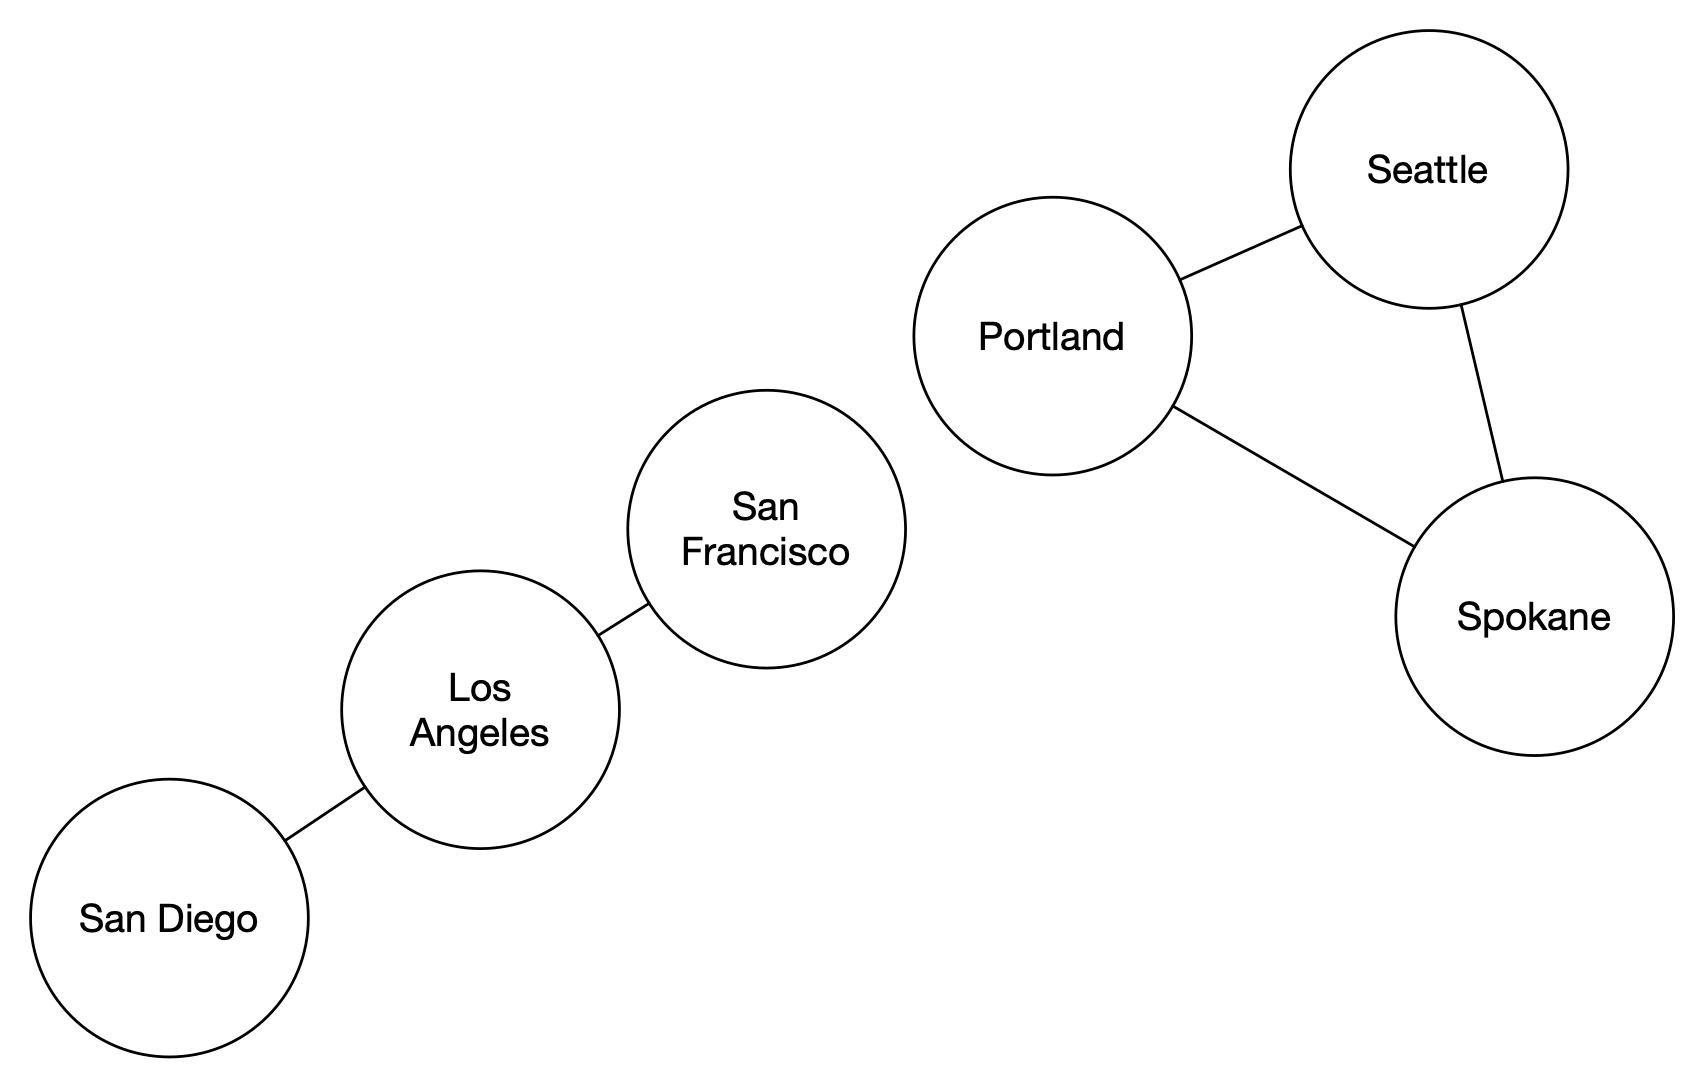
\includegraphics[width=0.7\textwidth]{notconnected.png}

This graph is \textit{not} connected! You can't follow edges from San Diego to Seattle.

In graph data, the nodes and edges often have attributes.  For
example, a node representing a city might have a name and a
population.  An edge representing a data line might have a bandwidth
(bits per second) and a latency (how many nanoseconds between when you
put a bit into the pipe and when it comes out the other end).

\section{Finding Good Paths}

For many problems, we are trying to find the best path from one
node to another.  If all the edges are the same, this usually means
finding the path that requires walking the fewest edges.

Sometimes the edges have a cost attribute.  For example, you might
want to find the cheapest way to ship a container from New York City
to Long Beach, California.  In this case the nodes are train depots.  Each
train line between the depots has a cost.  What is the cheapest path?

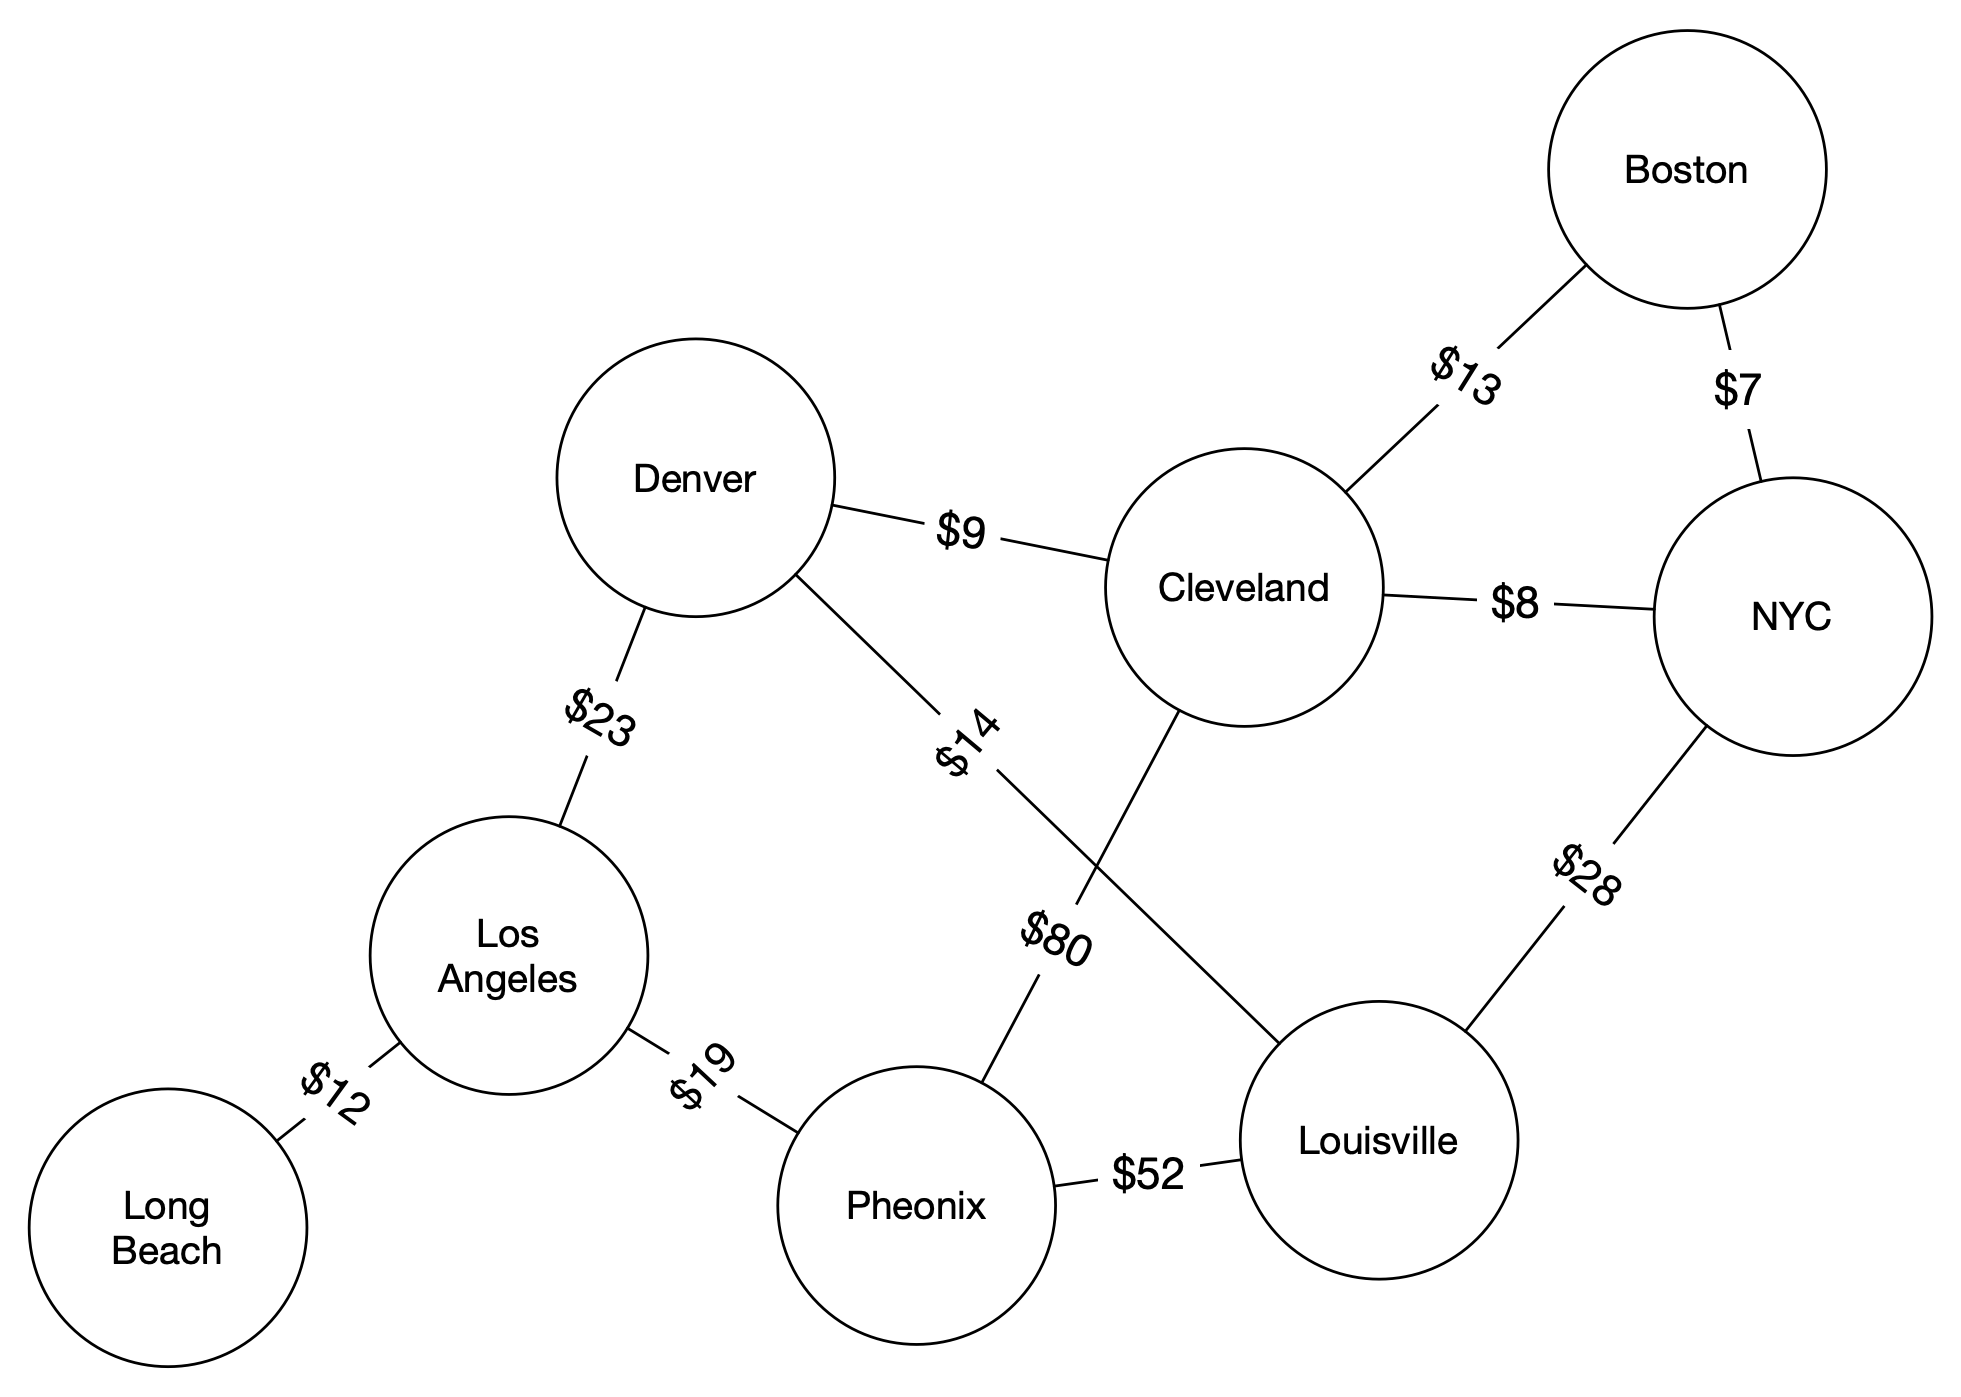
\includegraphics[width=0.7\textwidth]{depots.png}

When edges have costs like this,  we call the \newterm{weighted edges}.

The graphs that you see here are really small, so finding efficient
paths isn't difficult --- you could just try all of them! However, in
many computer programs, we are working with millions of nodes and
edges.  Efficient graph algorithms are \textit{really} important.

\section{Graphs in Python}

In this section you are going to write Python classes that will let
you represent an undirected graph with weighted edges, like the
shipping problem above.

(Naturally, things would look a little different if the graph were
directed or the edges were unweighted, but this is a good starting
place.)

Create a file called \filename{graph.py}.  This will hold the code for
your \pytype{Node} and \pytype{WeightedEdge} classes.  We will also
create a \pytype{Graph} class that will just hold onto the list of
its nodes.

\begin{itemize}
\item A \pytype{Node} will have a label string and a list of edges that touch it.
\item A \pytype{Edge} will have a cost and two nodes: \pyvar{node\_a} and \pyvar{node\_b}.
\item A \pytype{Graph} will have a list of nodes.
\end{itemize}

Here is what the object diagram would look like if you had only three cities:

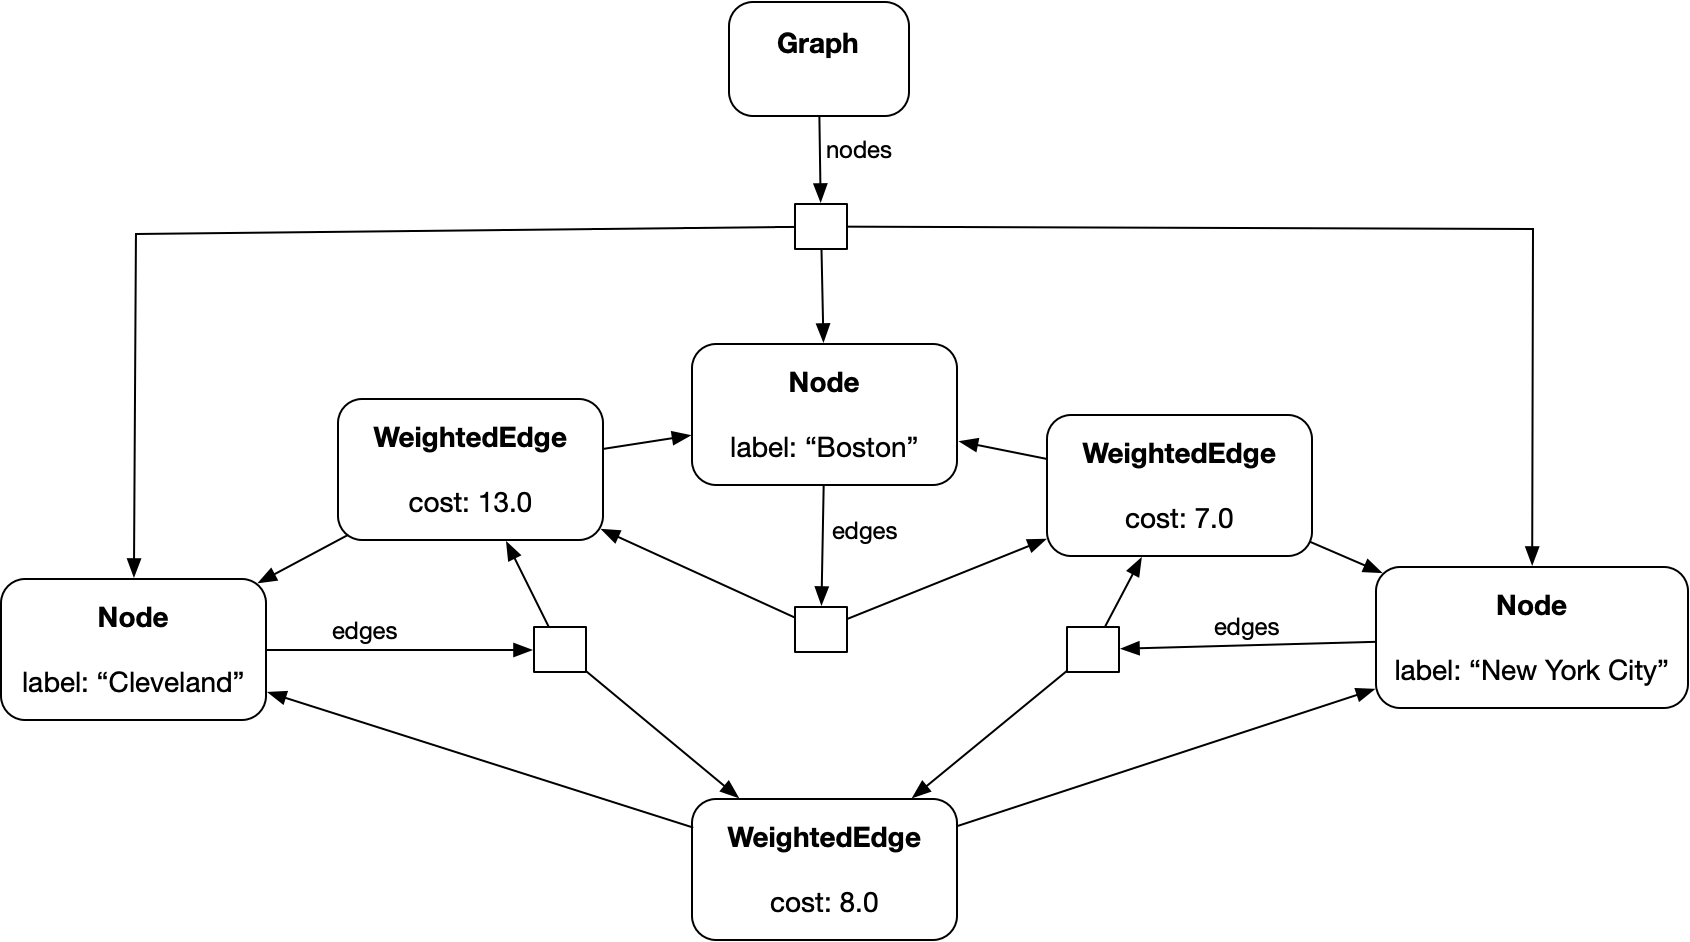
\includegraphics[width=0.8\textwidth]{objdiagram.png}

Put this code into \filename{graph.py}

\begin{verbatim}
class Node:
    def __init__(self, label):
        self.label = label
        self.edges = []

    def __repr__(self):
        return f"(node:{self.label}, edges:{len(self.edges)})"

class WeightedEdge:
    def __init__(self, cost, node_a, node_b):
        self.cost = cost
        self.node_a = node_a
        node_a.edges.append(self)
        self.node_b = node_b
        node_b.edges.append(self)

    def other_end(self, node_from):
        if self.node_a == node_from:
            return self.node_b
        else:
            return self.node_a

class Graph:
    def __init__(self):
        self.nodes = []

    def add_node(self, new_node):
        self.nodes.append(new_node)

    def __repr__(self):
        return f"(Graph:{self.nodes})"
\end{verbatim}

Now, let's create some instances of \pytype{Node} and
\pytype{WeightedEdge} and wire them together.  Create another file in
the same directory called \filename{cities.py}. Put in this code:

\begin{verbatim}
import graph

# Create an empty graph
network = graph.Graph()

# Create city nodes and add to graph
long_beach = graph.Node("Long Beach")
network.add_node(long_beach)
los_angeles = graph.Node("Los Angeles")
network.add_node(los_angeles)
denver = graph.Node("Denver")
network.add_node(denver)
pheonix = graph.Node("Pheonix")
network.add_node(pheonix)
louisville = graph.Node("Louisville")
network.add_node(louisville)
cleveland = graph.Node("Cleveland")
network.add_node(cleveland)
boston = graph.Node("Boston")
network.add_node(boston)
nyc = graph.Node("New York City")
network.add_node(nyc)

# Create edges
graph.WeightedEdge(12, long_beach, los_angeles)
graph.WeightedEdge(23.0, los_angeles, denver)
graph.WeightedEdge(19, los_angeles, pheonix)
graph.WeightedEdge(52, pheonix, louisville)
graph.WeightedEdge(14, denver, louisville)
graph.WeightedEdge(80, pheonix, cleveland)
graph.WeightedEdge(9, denver, cleveland)
graph.WeightedEdge(8, cleveland, nyc)
graph.WeightedEdge(28, louisville, nyc)
graph.WeightedEdge(7, nyc, boston)
graph.WeightedEdge(13, cleveland, boston)

print(network)
\end{verbatim}

Run it:
\begin{verbatim}
python3 cities.py
\end{verbatim}

You should see some rather unexciting output:

\begin{verbatim}
(Graph:[(node:Long Beach, edges:1), (node:Los Angeles, edges:3), (node:Denver, edges:3),
(node:Pheonix, edges:3), (node:Louisville, edges:3), (node:Cleveland, edges:4),
(node:Boston, edges:2), (node:New York City, edges:3)])
\end{verbatim}

But do not worry; we will make it more exciting in the next chapter!
